%---------------------------------------------
%build
%---------------------------------------------
\subsection{Build}
	\subsubsection{Syntax}
		\texttt{build(arg0, arg1:option, ...)}\\
		%\texttt{build([argument list])} \hl{is this a simpler way to write it?}
	
	\begin{phygdescription}
		{Builds initial graphs. The arguments of \texttt{build} specify the number of graphs 
		to be generated, and whether the build is based on \textit{distance} or \textit{character} 
		methods. Most options, with the exception of \texttt{rdWag}, an $O(n^3)$ distance based 
		option, are $O(n^2)$. Distance methods are considerably faster (lower constant 
		factor), but approximate in terms of character-based methods. Refinement, in the form 
		of branch swapping (\texttt{none}, \texttt{otu}, \texttt{spr}, and \texttt{tbr}) can be 
		specified within the command for distance builds. Refinement for character-based 
		Wagner builds occurs after the \texttt{build} process through \texttt{swap} and other
		refinement commands. Given the large time burden, distance refinement is usually 
		not time effective \citep{Wheeler2021}. \phyg does not replace trees previously 
		stored in memory.}
	\end{phygdescription}
		
	\subsubsection{Arguments}

	\begin{description}

		\item[block] Performs independent builds for each ``block'' of data. If this option 
		is not specified, the builds are performed combining all the data. Builds are performed 
		according 	to the other options (e.g. \texttt{character, distance}). The resulting tree 
		or \texttt{graph} is reconciled using the \texttt{eun} or \texttt{cun} commands. The 
		reconciled graph is resolved into display trees via the \texttt{displayTrees}, \texttt{first}, 
		and \texttt{atRandom} options. This option is especially useful for soft-wired network search. 
		Associated arguments of \texttt{block} include:
				
		\begin{description}
			\item[atRandom] When the option \texttt{block} is specified, this variable returns $n$ 
			display trees as specified by \texttt{displayTrees[:n]}, where trees are produced by 
			resolving network nodes uniformly at random. Compare with the \texttt{first} option, 
			which takes the ``first'' $n$ display trees resolved in arbitrary, but consistent, order.

			\item[block] Performs independent builds for each ``block'' of data.  These builds are combined
			into a single graph via \texttt{EUN} or \texttt{CUN} and returned as a graph (\texttt{graph}) and/or
			resolved display trees (\texttt{displaytrees})
			
			\item[cun] Reconciles \textbf {block} trees into a Cluster-Union-Network \citep{Baroni2005} 
			before resolution into display trees via the \texttt{displayTrees} or \texttt{atRandom} 
			options.
	
			\item[displayTrees[:n]] When the option \texttt{block} is specified, this variable 
			returns $n$ display trees specified by this optional argument. If the number of 
			display trees is not specified, up to $2^{63}$ may be returned.

			\item[eun] Reconciles block trees into a Edge-Union-Network \citep{MiyagiandWheeler2019, 
			Wheeler2022} before resolution into display trees via the \texttt{displayTrees} or 
			\texttt{atRandom} 
			options.

			\item[first] When the option \texttt{block} is specified, this variable specifies to 
			choose the first returns $n$ $n$ display trees resolved in arbitrary, but consistent, 
			order. Compare with 	\texttt{atRandom}.
			
			\item[graph] When the option \texttt{block} is specified, this variable returns the 
			reconciled graph as specified by \texttt{eun} or \texttt{cun}. The graph may be 
			altered to ensure that it is a ``phylogenetic'' graph sensu \cite{Moretetal2005}.
		\end{description}			
		
		\item [character] Performs random addition sequence Wagner \citep{Farris1970} builds 
		($O(n^2)$) for tree construction. If the graphtype is specified as softwired or hardwired 
		the resulting trees are rediagnosed as soft-wired graphs. This is 
		the default method for tree construction.
		
		\item [distance] Causes a pairwise distance matrix to be calculated ($O(n^2)$) and used 
		as a basis for distance tree construction. Specifies how the builds are refined (\texttt{none}, 
		\texttt{otu}, \texttt{spr}, \texttt{tbr}), as well as how the tree is constructed (\texttt{dWag}, 
		\texttt{nj}, \texttt{rdWag}, \texttt{wpgma}). Associated arguments of \texttt{distance} include:
				
		\begin{description}
			\item[best:n] Applies only to \texttt{rdWag}. Specifies the number of trees retained 
			after 	\texttt{rdWag} builds, selecting the best trees in terms of distance cost. The 
			options can be used to reduce the number of trees retained.  
			This number, $n$, of distance trees are rediagnosed as character trees
			and returned (limited by \texttt{return:m} below) for further analysis.
			
			\item[dWag] Performs distance Wagner build as in \citep{Farris1972} choosing the 
			`best' taxon to 
			add at each step, yielding a single tree. This method has a time complexity of $O(n^3)$.

			\item[nj] Performs Neighbor-Joining distance build \citep{Saitou1987}, yielding a single 
			tree. This method has a time complexity of $O(n^3)$.

			\item[none] No refinement (\texttt{otu}, \texttt{spr}, \texttt{tbr})) is performed after 
			distance builds. \texttt{none} is the default refinement method.
						
			\item[otu] Specifies that \texttt{otu} refinement \citep{Wheeler2021} is performed 
			after distance 
			builds.
			
			\item[rdWag] Performs randoms addition sequence distance Wagner builds, 
			yielding multiple trees determined by the argument \texttt{replicates:n}. This 
			method has a time complexity of $O(m \times n^2)$.
			
			\item[return:n] Limits the number of Wagner trees returned for further analysis.  By default
			all trees that are built (or limited by \texttt{best:m} in distance analysis) are returned.
			Limiting the number of returned trees (as opposed to simply generating that number) can result in
			a larger memory footprint.

			\item[spr] Specifies that \texttt{spr} refinement \citep{Dayhoff1969} is performed 
			after distance builds.

			\item[tbr] Specifies that \texttt{tbr} refinement \citep{Farris1988, swofford1990a} 
			is performed after distance builds.
		
			\item[wpgma] Performs Weighted Pair Group Method with Arithmetic Mean 
			distance build \citep{SokalandMichener1958}, yielding a single tree. This method 
			has a time complexity of $O(n^2)$.
		\end{description}

		\item [replicates:n] Applies to \texttt{rdWag} and \texttt{character}. Specifies the number of 
		random addition sequences performed.
	
	\end{description}		

	\subsubsection{Defaults}
		\texttt{build(character, replicates:10)}
		
	\begin{example}
	
		\item{\texttt{build(replicates:100)} \\
		Builds 100 random addition sequence character Wagner builds.}
		
		\item{\texttt{build(character, block, graph, cun, displaytrees:5, atrandom)}\\
		Builds 10 (the default) random addition sequence character Wagner builds, for each 
		block of data. The graph is reconciled into a Cluster-Union-Network, before resolution 
		into the 5 display trees. The trees are produced by resolving the network nodes 
		uniformly atRandom.}
		
		\item{\texttt{build(distance, rdWag, nj, wpgma)} \\ 
		Builds a single `best' addition sequence distance Wagner build, a Neighbor-Joining tree, 
		and a WPGMA tree. As the option \texttt{block} is not specified, the distance trees are 
		built using all the data.}
		
		\item{\texttt{build(distance, dWag, replicates:1000, best:10)}\\
		Builds 1000 distance Wagner builds and returns 10 of the lowest cost distance trees.}
	
		\item{\texttt{build(distance, rdwag, block, eun, displaytrees:3)}\\
		Builds 10 random addition sequence Wagner builds for each `block' of data. The graph 
		is reconciled into a Edge-Union-Network, before resolution into the 3 display trees. 
		The trees are produced by resolving the network nodes.}
		
		\item{\texttt{build(distance, block, rdWag, replicates:100, wpgma, best:10, otu)}\\
		Builds 100 random addition sequence distance Wagner builds, a WPGMA tree, 
		performs OTU swapping on the WPGMA and 10 of the lowest cost random addition 
		sequence Wagner trees. This distance search is performed on the `blocks' of data, 
		as opposed to all of the data.}

	\end{example}

%---------------------------------------------
%fuse
%---------------------------------------------
\subsection{Fuse}
	\subsubsection{Syntax}
		\texttt{fuse(option, option, ...)}
		
	\begin{phygdescription}
		{Performs Tree Fusing \citep{goloboff1999, moilanen1999, moilanen2001}. \texttt{fuse} 
		operates on a collection of graphs performing reciprocal graph recombination between 
		pairs of graphs. Non-identical subgraphs with identical leaf sets are exchanged between 
		graphs and the 	results evaluated. This process of exchange and evaluation continues 
		until no new graphs are found.
		This can be used in concert with other options to perform a Genetic Algorithm refinement
		\citep{Holland1975}. The behavior of \texttt{fuse} can be modified by the use of options 
		specifying SPR and TBR-like rearrangement of the combination process.}
	\end{phygdescription}
	
	\subsubsection{Arguments}
	\begin{description}
		\item [all]  During branch swapping-type operations, all rearrangement are tried before choosing a new graph. 
		
%		\item [alternate[:n]] Causes the exchanged subgraphs to be tried at multiple positions including rerooting of 
%		exchanged groups--alternating between SPR and TBR-type edits (up to optional 
%		$n$ edges aware from their initial positions).
		
		\item [atRandom] Chooses graphs to fuse uniformly at random when \texttt{pairs} is specified. 
		
		\item [best] Specifies the method for tree selection, which in this case returns the best graphs 
		found during fuse operations.		
		
		\item [keep:n] Limits the number of returned graphs to $n$. 
		
		\item [none] \hl{add description}
		
		\item [noReciprocal] Turns off \texttt{reciprocal}.
		
		\item [once] Performs a single round of fusing on input graphs and returns the resulting graphs. 
		Alternatively (and by default) fusing continues recursively until no new graphs are found.
		
		\item [pairs[:n]] Limits the number of graphs to be fused to $n$ pairs (as oppose to $\binom{m}{2}$ for $m$ graphs).
		
		\item [reciprocal] By default, fuse takes a subgraph of one graph in a pair and replaces the corresponding subgraph 
		in the other.  Reciprocal causes exchange and evaluation or graphs in both directions--roughly doubling time and 
		memory footprint.
		
		\item [spr[:n]] Causes the exchanged subgraphs to be tried at multiple positions (up to optional 
		$n$ edges aware from their initial positions).
		
		\item [steepest] During branch swapping-type operations, if a better graph is found, swapping shifts greedily to
		that graph. 
		
		\item [tbr[:n]] Causes the exchanged subgraphs to be tried at multiple positions (up to optional 
		$n$ edges aware from their initial positions) and with TBR-style rerooting of the exchanged 
		components.
		
		\item [unique] Specifies the method for tree selection, which in this case returns all unique 
		graphs found during fuse operations.	
	\end{description}	
	
	\subsubsection{Defaults}
		\texttt{fuse()} Keeps all the best graphs found, continues fusing until no new graphs are found. 
		No branch swapping style rearrangements are performed.
	
	\begin{example}
	
		\item{\texttt{fuse(best, once)}\\Fuses input graphs and returns best graphs after a single round of 
		fusing.}
		
		\item{\texttt{fuse(tbr, keep:10)} \\Fuses input graphs and preforms TBR-style replacement and 
		rerooting of pruned components returning up to 10 best cost graphs.}
		
	\end{example}

%---------------------------------------------
%read
%---------------------------------------------	
\subsection{Read}
	\label{subsec:Read}
	\subsubsection{Syntax}
		\texttt{read(option:"filename", option:"filename", ...)}
			
	\begin{phygdescription}
		{Imports file-based information, including data files, tree and graph files. \texttt{read} 
		commands must contain an input file. Supported data formats include FASTA, FASTC
		xand TNT files, and graph formats include Dot, Enewick, Fenewick, and Newick. 
		Filenames must be included in quotes. Filenames must include the appropriate suffix (e.g. .fas, 
		.ss, .mat). The exclusion of these suffixes will result in an error. The filename must
		match exactly, including capitalization. \phyg will attempt to recognize the type of input
		and parse appropriately. Otherwise, the type of file can be indicated, using one of the 
		options below. The options prepend 	the filename with a colon (`:') and will modify the 
		processing of the input file. Prepending the file type prevents any ambiguity when the 
		file is parsedThis command can also use wildcard expressions (`*', `?'), 
		which can be useful when reading in multiple files of the same type.}
	\end{phygdescription}

	\subsubsection{Arguments}
	
	\begin{description}
		\item [aminoacid:] Specifies that the file contents are parsed as IUPAC coded amino 
		acid data in fasta \citep{PearsonandLipman1988} format.

		\item [block:] Specifies that the file contains block %\hl{ref?} 
		information. Each line contains 
		the new block name followed by names of input files to be assigned to that data block. 
		Blocks are initially named as the input file name with ``:0'' appended. In the examples, 
		data from files ``b'' and ``c'' will be assigned to block ``a''. There can be no spaces in 
		file or block names.
			
			\begin{quote}
					\texttt{"a" "b:0" "c:0"}
			\end{quote}
	
		\item [dot:] Specifies that the file contains a graph in `dot' format for use with graph 
		rendering software such as \href{https://en.wikipedia.org/wiki/Graphviz}{GraphViz}.
			
		\item [enewick:] Specifies that the file contains Enhanced Newick format graph(s) as
		specified here \citep{Cardonaetal2008}. 
			
		\item [exclude:] Specifies that the file contains the names of terminal taxa to be 
		excluded from an analysis. Taxa appear in the form of a list, with a single taxon per 
		line. Thus, taxa not included in the list and present in input files, will be included in 
		analysis. Compare with \texttt{include}.
			
		\item [fasta:] Ensures that file contents are parsed in fasta \citep{PearsonandLipman1988}
		format. This is used for single character sequences such as binary streams, IUPAC 
		nucleotide and amino acid sequence data.
			
		\item [fastc:] Ensures that file contents are parsed in fastc \citep{WheelerandWashburn2019}
		format. This is used for multi-character sequences such as gene synteny, developmental, 
		or linguistic data.
			
		\item [fenewick:] Specifies that the file contains Forest Enhanced Newick format graph(s)  
		specified \href{https://www.github.com/wardwheeler/euncon}{here} \citep{Wheeler2022}.
			
		\item [include:] Specifies the names of terminal taxa to be included in the analysis. 
		Taxa appear in the form of a list, with a single taxon per line. It is possible to specify 
		terminals that have no data. This may be done in order to diagnose a large tree on 
		partial data. If there are no data for a leaf taxon, a warning will be printed to \texttt{stderr}. 
		Taxa not included in this list, but present in the inputted data files, will be excluded from 
		the analysis. Compare with \texttt{exclude}.
			
		\item [newick:] Specifies that the file contains Newick format graph(s) as specified 
		\href{https://evolution.genetics.washington.edu/phylip/newick_doc.html}{here}.
			
		\item [nucleotide:] Ensures that file contents are parsed as IUPAC coded nucleotide data 
		in fasta \citep{PearsonandLipman1988} format.
			
		\item [preaminoacid:] Specifies that the file contents are parsed as IUPAC coded amino 
		acid data in  prealigned fasta \citep{PearsonandLipman1988} format, leaving 
		gap characters (``-'') in the sequences and alignment correspondences are not re-examined.
		
		\item [prefasta:] Specifies that the sequences are prealigned in a fasta format, leaving 
		gap characters (``-'') in the sequences and alignment correspondences are not re-examined. 
		This option exists to ensure proper parsing (and in case auto-format detection is incorrect).
		Prealigned fasta files \textbf{must} be of the same length.
			
		\item [prefastc:] Specifies that the sequences are prealigned in a fastc format, leaving gap 
		characters (``-'') in the sequences and alignment correspondences are not re-examined. 
		This option exists to ensure proper parsing (and in case auto-format detection is incorrect).
		Prealigned fastc files \textbf{must} be of the same length.			
		
		\item [prenucleotide:] Ensures that file contents are parsed as IUPAC coded nucleotide data 
		in fasta \citep{PearsonandLipman1988} format, leaving 
		gap characters (``-'') in the sequences and alignment correspondences are not re-examined.
		
		\item [rename:] Replaces the name(s) of specified terminals in the file. This command allows 
		for substituting taxon names and can help merge multiple datasets without modifying the 
		original data file. The file contains a series of lines, each of which contains at least two strings. 
		The first string (input taxon name) will replace the second and all subsequent strings (taxon 
		names) on that line. In the example given in Figure \ref{renamefile} the taxon Hydrus\_granulatus 
		will be renamed as Acrochordus\_granulatus, the taxa Gloydius\_boehmei and Gloydius\_mogoi
		will be renamed as Gloydius\_halys and the taxa Crotalus\_mutus, Scytale\_catenatus and 
		Coluber\_crotalinus will be renamed as Lachesis\_muta.
		
		\begin{figure}
		\centering
		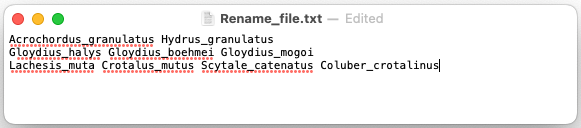
\includegraphics[width=0.8\textwidth]{Rename_file.jpg}
		\caption{Renaming text file containing the lists of terminal taxa to be renamed.}
		\label{renamefile}
		\end{figure}
		
		The \texttt{rename} function can also be specified as a command, see \texttt{rename}
		(Section \ref{subsec:Rename}).
					 
		\item [tcm:] This refers to a file containing a custom-alphabet matrix that specifies varying 
		costs among alphabet elements in a sequence. The elements in the alphabet can be letters, 
		digits, or both. \\
		The \texttt{tcm} contains two parts: the first line of the file contains the alphabet elements 
		separated by a space and the transformation cost matrix, which follows below. The dash 
		character representing an insertion/deletion or indel character is not specified on the first 
		line of the file, but added to the alphabet automatically. The second part is the \texttt{tcm}, 
		which is a square matrix with $n + 1$ elements ($n$ is the size of the alphabet). 
		The positions from left to right and top to bottom in this matrix correspond to the sequence 
		of the elements as they are listed in the alphabet. An extra rightmost column and lowermost
		row correspond to indel (gap) costs to and from alphabet elements. At present, this matrix 
		must be symmetrical, but not necessarily metric. Non-metric tcm's can yield unexpected 
		results. Transformation costs must be integers. If real values are desired, a character can 
		be weighted with a floating point value factor. \\
		For a sequence with four elements alpha, beta, gamma and delta and an indel cost of 4 
		for all insertion deletion transformations, a valid custom alphabet file is provided below:
		\\
		\begin{equation*}
		%\nolabel
		\begin{array}{lllll}
		alpha & beta & gamma & delta &  \\
		0 &   2 &  1 &   2 &   5 \\
		2 &   0 &  2 &   1 &   5 \\
		1 &   2 &  0 &   2 &   5 \\
		2 &   1 &  2 &   0 &   5 \\
		5 &   5 &  5 &   5 &   0
		\end{array}
		\end{equation*} 
		\\
		In this example, the cost of transformation of \texttt{alpha} into \texttt{beta} is \texttt{2},
		and cost of a deletion or insertion of any of the four elements costs \texttt{5}.

		\item [tnt:] Ensures that file contents are parsed in TNT \citep{Goloboffetal2008} format. 
		Not all TNT data commands are currently supported. To ensure that the file is correctly
		parsed, the file must begin with \texttt{xread}, followed by an optional comment in single 
		quotes ('this is a comment'), followed by the number of characters and taxa. The data 
		follow on a new line. Taxon names are followed by state data. Data may be in multiple 
		blocks (interleaved) or in sequential format. These interleaved blocks may consist of a 
		series of single character states without spaces between them, or multiple (or single) 
		character states (e.g. \texttt{alpha}) with space between the individual codings. Blocks 
		must be of all one type (ie. single character codings without spaces, or multi-character 
		separated by spaces). The data block \textit{must} be followed by a single semicolon 
		(``;'') 	on its own line.\\
			
		The character settings (i.e. \texttt{ccode} commands) follow the data block, beginning 
		on a 	new line. These character settings always terminate with a semi-colon (\texttt{;}). 
		These settings include: activate (\texttt{[}) or deactivate (\texttt{]}); make additive/ordered 
		(\texttt{+}) 	or non-additive/unordered (\texttt{-}); apply step-matrix costs (\texttt{(}) with 
		scopes (e.g. \texttt{cc + 10 12;} and  \texttt{cc (.; costs 0 = 0/1 1 0/2 2 0/3 3 0/4 4 1/2 1 
		1/3 2 1/4 3 2/3 1 2/4 2 3/4 1;}) including abbreviated scopes (\texttt{cc -.;}). %\hl{what about ) make additive or non-additive again?} 
		There may 
		be multiple character setting statements in a single line. Character settings must be 
		followed by \texttt{proc/;} on its own line. \texttt{PhyG} will not process
		any file contents that follow \texttt{proc/;}.
		  
		 Additive/ordered character states must be numbers (integer or floating point). Ranges 
		 for continuous characters are specified with a dash within square brackets (e.g. 
		 \texttt{[1-2.1]}). Character state polymorphism are specified in square brackets without 
		 spaces for single character states (e.g. \texttt{[03]}), and with spaces for multi-character 
		 states. %(e.g. \hl{\texttt{[???}}).
		  
		 Dashes in multi-character states (e.g. \texttt{Blue-ish}) 
		 are treated as part of the character state specification. If the user wishes that dashes 
		 be treated as missing data (`?'), the file must be edited to reflect this by replacing the 
		 dashes that are to be treated as missing data with question 
		 marks (`?').
		  
		  Example file:
		  	\begin{quote}
			  	\texttt{xread\\
				  	`An example TNT file' 8 5\\
				  	A 000\\
				  	B a14\\
				  	C b22\\
				  	D ?33\\
				  	E d[01]4\\}
			  	
			  	\texttt{A Blue-ish -\\
				  	B Green-ish OneFish\\
				  	C Rather-Red TwoFish\\
				  	D Almost-Cyan RedFish\\
				  	E Orange-definitely BlueFish\\}
					
				\texttt{A 5.2 - ?\\
					 B 5.3 0.3 1.1\\
					 C 3.2 0.1 1.1\\
					 D 5.2 1.1 0.1\\
					 E 5.1 1.1 0.1\\
				  	;\\
				  	cc .;\\
				  	cc + 2;\\
				  	proc/;\\}
			  \end{quote}
	\end{description}	
		
	\subsubsection{Defaults}
		\texttt{read("fileName")} reads data from fileName and attempts to recognize the 
		file type and parse accordingly. The assumed file type is printed to \texttt{stderr} for 
		verification.
		
	\begin{example}
		
		\item{\texttt{read(prefasta:"myDnaSequenceFile.fas")}\\ Reads sequence data from 
		``myDnaSequenceFile.fas'' as prealigned data.}
		
		\item{\texttt{read(rename:"myRenameFile")}\\ Reads a list of taxa and names to be 
		assigned.} 
		
	\end{example}
		
%---------------------------------------------
%reblock
%---------------------------------------------
\subsection{Reblock}
	\subsubsection{Syntax}
		\texttt{reblock("newBlockName", "inputFile0", "inputFile1",...)}
	
	\begin{phygdescription}
	{Assigns input data to ``blocks'' that will follow the same display tree when optimized
	as ``soft-wired'' networks. By default, each input data file is assigned its own block with 
	the name of the input file. The \texttt{block} command is used to reassign these data to 
	new, combined blocks. Spaces are not allowed in block names and will produce 
	\texttt{unrecognized block name} errors.} 
	\end{phygdescription}
	
	\subsubsection{Arguments}
		The first argument is the block to be created, the remainder are the input data to 
		be assigned to that block. Blocks are initially named as the input file name with 
		``:0'' appended. Blocks are reported in \texttt{report(data)} command.
	
	\subsubsection{Defaults}
		None.
	
	\begin{example}

		\item{\texttt{reblock("a","b\#0","c\#0")}\\ Assigns input data from file ``b'' and ``c'' 
		to block ``a''. }
	
	\end{example}

%---------------------------------------------
%refine
%---------------------------------------------		
\subsection{Refine}
	\subsubsection{Syntax}
		\texttt{refine(option, option,...)}
		
	\begin{phygdescription}
		{Performs edit operations (addition, deletion, move) on network edges, and therefore
		only applies to soft-wired and hard-wired graphs.}
	\end{phygdescription}

	\subsubsection{Arguments}
		
		\begin{description}
		\item[annealing[:n]] Specifies that $n$ (default 1) rounds of simulated annealing optimization 
		\citep{Metropolisetal1953, Kirkpatricketal1983, Cerny1985} are performed in concert with 
		\texttt{netAdd}, \texttt{netDel}, and \texttt{netMove}. The acceptance of candidate graphs is 
		determined by the probability $e ^ {- (c_c - c_b)/ (c_b * (k_{max} -k)/ k_{max})}$, where $c_c$ 
		is the cost of the candidate graph, $c_b$ is the cost of the current best graph, $k$ is the step 
		number, and $k_{max}$ is the maximum number of steps (set by the \texttt{steps:m}, default 10) 
		option.
		
			\begin{description}
		
			\item[netadd] Adds network edges to existing input graphs at all possible positions until no 
			better cost graph is found.
			
			\item[netdel] Deletes network edges from input graphs one at a time until no better cost 
			graph is found.
			
			\item[netmove] Moves existing network edges in input graphs one at a time to new positions 
			until no better cost graph 
			is found.
			
			\item[steps:n] Specifies that $n$ (default 10) temperature steps are performed during 
			simulated 
			annealing (as specified by the \texttt{annealing}) option.

			\end{description}

			
		\item[drift[:n]] Specifies that $n$ (default 1) rounds of the ``drifting'' form of simulated annealing 
		\citep{goloboff1999} optimization are performed in concert with \texttt{netAdd}, 	\texttt{netDel}, 
		and \texttt{netMove}. The acceptance of candidate graphs is determined by the probability 
		$1/ (wf + c_c - c_b)$, where $c_c$ is the cost of the candidate graph, $c_b$ is the cost of the 
		current best graph, and $wf$ is the \texttt{acceptWorse} (set by the \texttt{acceptWorse:m}, 
		default 1.0) option. Equal cost graphs are accepted with probability set by the \texttt{acceptEqual} 
		option. \texttt{Drift} differs from \texttt{annealing} in that there are no cooling steps to modify 
		acceptance probabilities. The maximum number of graph changes is set by \texttt{maxChanges}
			
					
		\item[geneticAlgorithm or ga] Performs Genetic Algorithm \citep{Holland1975} refinement in 
		concert with the options \texttt{generations}, \texttt{popsize}, \texttt{severity}, and 
		\texttt{recombinations}. 
			
			\begin{description}
		
			\item[generations:[n]] Specifies the number of generations (sequential iterations) for 
			\texttt{geneticAlgorithm}. The default is $n=10$.

			\item[popsize:[n]] Specifies the population size for \texttt{geneticAlgorithm}. The default is 
			$n=20$.
			
			\item[recombinations:[n]] Specifies the number of recombination (fusing) events for 
			\texttt{geneticAlgorithm}. The default is $n=100$.
			
			\item[severity:[n]] Specifies the severity of selection against sub-optimal graph solutions 
			events for \texttt{geneticAlgorithm}. The higher the value, the less severe the penalty. The 
			default is $n=1.0$.
			
			\item[stop:n] Causes the \texttt{geneticAlgorithm} to terminate after $n$ generations without 
			improvement in graph cost.  Default is to only terminate when the number generations has 
			been completed.

			\end{description}
		
		\item[keep:n] Limits the number of returned graphs to $n$. 
		
		\end{description}
	
	%add defaults and examples	
%---------------------------------------------
%rename
%---------------------------------------------	
\subsection{Rename}
	\label{subsec:Rename}
	\subsubsection{Syntax}
		\texttt{rename("newName", "oldName1", "oldName2",...)}
		
	\begin{phygdescription}
	{Replaces the name(s) of specified terminals. 
	The command consists of a terminal identifier followed by a comma and then by either 
	a string containing a pair (or pairs) of strings containing the names of items being renamed.
	The first string (name) is assigned to taxa with the strings (names) that follow. This can be 
	useful when combining data from different sources, such as GenBank, or in revising names 
	to reflect taxonomic changes. Irrespective of where this command appears in the script file, 
	\phyg will execute this command prior to importing the data files. Compare with the 
	argument \texttt{rename} of the command \texttt{read} (Section \ref{subsec:Read}).
	In the example below, the taxa ``b'' and ``c'' will be renamed to ``a''.

	\begin{quote}
	rename("a","b","c")
	\end{quote}}
	\end{phygdescription}
	
	\subsubsection{Arguments}
		Taxon names to assign and be assigned.
		
	\subsubsection{Defaults}
		None.
		
	\begin{example}
	
		\item{\texttt{rename("a","b","c")}\\ Renames ``b'' and ``c'' to ``a''. }
				
	\end{example}


%---------------------------------------------
%report
%---------------------------------------------				
\subsection{Report}
	\subsubsection{Syntax}
		\texttt{report("filename", arg0, arg1,...)}
	
	\begin{phygdescription}
		{Outputs the results of the current analysis to a file or to \texttt{stderr}. To redirect the 
		output to a file, the file name (in quotes), followed by a comma, must be included in 
		the argument list of report. All arguments for \texttt{report} are optional. This command 
		allows the user to output information concerning the characters and terminals, 
		diagnosis, export static homology data, implied alignments, trees, graphs, dot files, 
		as well as other miscellaneous arguments. By default, new information printed to 
		a file is appended to the file. The option \texttt{overwrite} overrides the default and 
		rewrites the file. Many of the report options can be output in csv format,  which can
		subsequently be imported into spreadsheet programs.}
	\end{phygdescription}
	
	\subsubsection{Arguments}
	\begin{description}
		
		\item[crossrefs] Reports a table with terminals represented in rows, and the data files in 
		columns. A plus sign (``+'') indicates that data for a given terminal is present in the 
		corresponding file; a minus sign (``--'') indicates that it is absent. It is highly recommended 
		that the user use this report option to examine the data, having imported them into \phyg. 
		This argument is a useful tool for visual representation of missing data, as well as highlight 
		inconsistencies in the spelling of taxon names in different data files. The reported file is 
		in csv format.
			
		\item[data] Outputs a summary of the input data. More specifically, \phyg will report 
		aspects of the input data. 
		%\hl{"Index","Block","Name","Type","Activity","Weight","Prealigned","Alphabet","TCM"}
	
		\item[diagnosis] Outputs graph diagnosis information such as vertex and states and edge 
		statistics in csv format. 
		
		\item[displaytrees] Outputs graph information for soft-wired networks. The ``display'' trees 
		are output for each data block. 
		
		\item[graph] Outputs a graph in format specified by the other arguments in the command. 
		These are \texttt{dot} for 
		GraphViz graph format, \texttt{dotpdf} for pdf (or ps for OSX), \texttt{newick} for Newick, 
		ENewick, or ForestEnewick depending on the graph type, \texttt{ascii} for an ascii rendering. 
		In order to output pdf files (via \texttt{dotpdf}) ``dot'' must be installed from 
		\url{https://graphviz.org/download/}. PhyG will not error, but output a ``dot'' file that 
		can be processed later.
		
		\item[pairdist] Outputs a taxon pairwise distance matrix in csv format. 
		
		\item[reconcile] Outputs a single ``reconciled'' graph from all graphs in memory. The 
		methods include consensus, supertree, and other supergraph methods as described in 
		\cite{Wheeler2012, Wheeler2022}. When \texttt{reconcile} is specified as a command 
		option a series of other options may be specified to tailor the desired outputs:
			\begin{description}
			\item [Method:eun$\mid$cun$\mid$majority$\mid$strict$\mid$Adams] 
			This commands specifies the type of output graph. EUN is the Edge-Union-Network 
			\citep{MiyagiandWheeler2019}, CUN the Cluster Union Network \citep{Baroni2005},
			majority (with fraction specified by `threshold') specifies that a values between 0 and 
			100 of either vertices or edges will be retained. If all inputs are trees with the same leaf 
			set this will be the Majority-Rule Consensus \citep{MargushandMcMorris1981}.
			Strict requires all vertices be present to be included in the final graph. If all inputs are 
			trees with the same leaf set this will be the Strict Consensus \citep{Schuhandpolhemus1980}. 
			Adams denotes the Adams II consensus \citep{Adams1972}.\\
			Default:eun.
							
			\item [Compare:Combinable$\mid$identity] Specifies how group 
			comparisons are to be made. Either by identical match [(A, (B,C))$\neq$(A,B,C)],
			combinable sensu \cite{Nelson1979} [(A, (B,C)) consistent with (A,B,C)]. This option 
			can be used to specify ``semi-strict'' consensus \citep{Bremer1990}.\\
			Default:combinable.
							
			\item [Threshold:(0-100)] Threshold must be an integer between 0 and 100 
			and specifies the frequency of vertex or edge occurrence in input graphs to be included 
			in the output graph. Affects the behavior of `eun' and` majority'.\\
			Default:0.
			
			\item [Connect:True$\mid$False] Specifies the output graph be connected 
			(single component), potentially creating a root node and new edges labeled with ``0.0''.\\
			Default:True.
			
			\item [EdgeLabel:True$\mid$False] Specifies the output graph have edges 
			labeled with their frequency in input graphs. \\
			Default:True.
			
			\item [VertexLabel:True$\mid$False] Specifies the output graph have vertices 
			labeled with their subtree leaf set.\\
			Default:False.
	
			\item [OutFormat:Dot$\mid$FENewick] Specifies the output graph format 
			as either Graphviz `dot' or FEN. \\ 
			Default:Dot.
			\end{description}	
				
		\item[support] Outputs support graphs. Resampling graphs are independent of the 
		input graphs while Goodman-Bremer are based on current graphs. Multiple formats 
		can be output via additional options including \texttt{dot} for GraphViz graph format, 
		\texttt{dotpdf} for pdf (or ps for OSX), \texttt{newick} for Newick, ENewick, or 
		ForestEnewick depending on the graph type, \texttt{ascii} for an ascii rendering. 
		In order to output pdf files (via \texttt{dotpdf}) ``dot'' must be installed from 
		\url{https://graphviz.org/download/}. \phyg will not error, but output a ``dot'' file that 
		can be processed later.
		
		\item[search] Outputs search statistics in csv format.
		 
	\end{description}			
		
	\subsubsection{Defaults}
		\texttt{report()} prints input data and output graph diagnosis to stderr. Default graph 
		representation is \texttt{dot}.
		
	\begin{example}
		\item{\texttt{report("outFile", newick, overwrite)}\\ Outputs graphs in newick format to 
		``outFile'', overwriting any existing information.}
		
		\item{\texttt{report("outFile", crossrefs)}\\ Outputs presence/absence for taxa in input files. 
		A `+' is output if taxa are present in an input data file, and `-' if. File is in csv format. This 
		can be useful in checking for missing sequence or other data and expected renaming.}
		
		\item{\texttt{report("outFile", dot, reconcile, method:eun, threshold:51)}\\ Outputs reconciled 
		graph using the Edge-Union-Network method with a minimum edge frequency of 51\% in 
		dot format to ``outFile'', appending to any existing information in ``outFile''.}
	\end{example}

%---------------------------------------------
%run
%---------------------------------------------		
\subsection{Run}
	\subsubsection{Syntax}
		\texttt{run("filename")}
		
	\begin{phygdescription}
		{Used to execute a \phyg script file containing commands. The script filename must be 
		included in quotes. 
		Executing scripts using \texttt{run} can be useful to specify common actions such as file inputs 
		and graph construction. }
	\end{phygdescription}
	
	\subsubsection{Arguments}
		The only argument is the filename containing commands to be executed.
		
	\subsubsection{Defaults}
		There are no default settings of \texttt{run}. 
	
	\begin{example}
		\item{\texttt{run("readFiles.pg")}\\ Executes "readFiles.pg", which may contain multiple input 
		files to be \texttt{read}.}
		
		\item{\texttt{run("searchCommands.pg")}\\ Executes "searchCommands.pg", which may 
		contain commands defining a common search strategy (e.g. \texttt{build}).}
	\end{example}

%---------------------------------------------
%search
%---------------------------------------------		
\subsection{Search}
	\subsubsection{Syntax}
		\texttt{search(arg0:option, arg1:option, ...)}
	
	\begin{phygdescription}
		{This command implements a default search strategy, performing a timed randomized 
		series of graph optimization methods including building, swapping, recombination (fusing), 
		simulated annealing and drifting, network edge addition/deletion/moving, and Genetic 
		Algorithm. The parameters and order for this search are randomized. The arguments 
		specify the number independent instances of search (\texttt{instances}, default 1), and duration 
		(\texttt{days}, \texttt{hours}, \texttt{minutes}, and \texttt{seconds}; 
		\hl{default 30 seconds}). Successive rounds of search gather 
		any solutions from previous sequential or parallel rounds as well as any input graphs.
		Since search methods may vary in how long they take, individual iterations may take 
		longer that the specified duration.  By default, search strategies are chosen uniformly at random, 
		if \texttt{Thompson} is specified, Thompson sampling \cite{Thompson1933,WheelerThompson} 
		is used to modify the probabilities of search strategies over the search duration.
		
		When performing a \texttt{search} it is important to set the amount of time, such that the 
		program has a reasonable amount of time to perform a search. Therefore, it is important
		to have some idea as to the length of time it would take to do a single round of searching.
		\hl{how reasonable is this expectation of the user?}}
	\end{phygdescription}
			
	\subsubsection{Arguments}
	\begin{description}
		\item[days:n] Adds $n$ 24 hour days to search time.
		
		\item[hours:n] Adds $n$ hours to search time.
		
		\item[instances:n] Specifies $n$ (potentially parallel) search instances.
		
		\item[keep:n] Keeps up to $n$ graphs.
		
		\item[maxNetEdges:n] Limits maximum number of network edges to $n$. Only to be used if
		soft-wired or hard-wired graphs.
		
		\item[minutes:n] Adds $n$ minutes to search time.
		
		%\item[seconds:n] Adds $n$ seconds to search time.
		
		\item[stop:n] Specifies that the search will be terminated after $n$ iterations without 
		improving the best graph cost. Should this argument be used with a specific time strategy, 
		whichever comes first, the search will end.
		
		\item[Thompson] Specifies that randomized choice of search option (e.g. Wagner 
		Build, SPR, Genetic Algorithm) 
		employs Thompson sampling.
		\begin{description}
			\item[mFactor:n] Specifies the memory factor $n$ for Thompson sampling. Parameter
			for linear and exponential.
		
			\item[linear] Specifies that the Thompson memory is a linear function of \texttt{mFactor}, 
			$m$.  Updating of search type, $\theta^k$, probability for iteration $n$ is $\frac{m}{m+1} 
			\theta^k_{n-1} + \frac{1}{m+1} \theta^k_n$.  Thompson success is a function of whether 
			a search was successful in reducing the graph cost and how long that search took to 
			complete.
		
			\item[exponential] Specifies that the Thompson memory is an exponential function of 
			\texttt{mFactor}, $m$.  Updating of search type, $\theta^k$, probability for iteration 
			$n$ is $ \left(1 - \frac{1}{2^m} \theta^k_{n-1}\right) + \left(\frac{1}{2^m} \theta^k_n \right)$.  
			Thompson success is a function of whether a search was successful in reducing the graph 
			cost and how long that search took to complete.
		\end{description}	

	\end{description}
		
	\subsubsection{Defaults}
		\texttt{search()} Performs 1 instance of \hl{30 seconds} keeping up to 10 graph}.
		
	\begin{example}
		\item{\texttt{search(hours:10, instances:2)}\\ Performs 2 search instance (in parallel if the 
		program is executed in parallel) for 10 hours each.}
				
		\item{\texttt{search(hours:10, minutes:30)}\\ Performs a single search instance for 10 
		hours and 30 minutes.}
	\end{example}
	
%---------------------------------------------
%select
%---------------------------------------------		
\subsection{Select}
	\subsubsection{Syntax}
		\texttt{set(arg0:option, arg1:option, ...)}
	
	\begin{phygdescription}
		{Specifies the method and number of graphs to be saved at any point. When multiple 
		graphs are present, the \texttt{select} command will specify which of the graphs to keep 
		for further analysis or reporting.}
	\end{phygdescription}
				
	\subsubsection{Arguments}
		\begin{description}
			\item[all] Keeps all graphs.
		
			\item[best:n] Selects and keeps the graphs with the best optimality value.
			
			\item[atRandom] Keeps graphs chosen at random.
			
			\item[threshold:f] Keeps unique graphs up to fraction \texttt{f} longer than shortest graph.  
			\texttt{f} is a floating point number (e.g. 0.1) and should be greater than 0.
			
			\item[unique:n] Keeps up to \texttt{n} unique graphs, which may not necessarily be the 
			best graphs.
		\end{description}

	\subsubsection{Defaults}
		\texttt{select()} Keeps all unique graphs of best optimality value.
		
	\begin{example}
		\item{\texttt{select(random:10)}\\ Keeps up to 10 graphs, selected at random.}
						
		\item{\texttt{select(best:10)}\\ Keeps up to 10 graphs of best optimality value.}
	\end{example}

%---------------------------------------------
%set
%---------------------------------------------				
\subsection{Set}
	\subsubsection{Syntax}
		\texttt{set(arg0:option, arg1:option, ...)}
	
	\begin{phygdescription}
		{Changes the settings of \phyg. This command performs an array of functions
		from specifying the seed of the random number generator, to selecting a terminal for
		rooting output trees, to specifying  graph type, final assignment, and 	optimality 
		criterion. All \texttt{set} commands are executed at the start of a run, irrespective of
		where they appear in the script. The command \texttt{transform} is used to modify 
		global settings during a run (see \texttt{transform} Section \ref{subsec:Transform}).}
	\end{phygdescription}
			
	\subsubsection{Arguments}
		\begin{description}
%			\item[compressResolutions:True|False] %\hl{change to BOOL} 
%			Determines whether soft-wired graph resolutions are ``compressed'' if multiple 
%			vertex assignments in alternate display trees are equal in subtree leaf set, only 
%			the first lowest cost resolution is retained. This option can significantly reduce 
%			the time to evaluate softwired graphs, but can increase the optimality score of 
%			the graph. This can be used in combination with \texttt{transform(compressResolutions:True)} 
%			or \texttt{transform(softwiredMethod:\\Exhaustive)} 
%			at a later stage to improve graph score.
			
%			\item[criterion:parsimony|mapa|pmdl] 
			\item[criterion:parsimony|mapa] 
			Sets the optimality criterion for graph search to be 
			method. Currently, parsimony and MAPA \citep{Wheeler2014} 
%			and PMDL \citep{WheelerandVaron2022} 
			are supported.
			
			\item[finalAssignment:DirectOptimization|DO|ImpliedAlignment|IA] Sets the method 
			of determining the ``final'' sequence states. DirectOptimization (DO) uses soft-wire the DO 
			method to assign the final states, which is more time consuming than \texttt{ImpliedAlignment}. 
			DO has an additional factor of potentially $O(n^2)$ in sequence length compared 
			to the constant factor for IA due to additional graph traversals.
			
%			\item[graphFactor:nopenalty|W15|W23|PMDL] Sets the network penalty for a soft-wired network\\ 
%			(\texttt{W15}),  (\texttt{W23}), or \texttt{PMDL} (for criterion = PMDL). W15 employs the
%			parsimony network penalty of \cite{Wheeler2015}. W23 sets the parsimony network penalty akin to
%			W15, but with the penalty applied to all blocks (more severe).
			
			\item[graphFactor:nopenalty|W15|W23] Sets the network penalty for a soft-wired network\\ 
			\texttt{NoPenalty}, (\texttt{W15}),  or (\texttt{W23}). W15 employs the
			parsimony network penalty of \cite{Wheeler2015}. W23 sets the parsimony network penalty akin to
			W15, but with the penalty applied to all blocks (more severe).
			
			\item[graphsSteepest:n] Sets the maximum number of graphs to be evaluated 
			simultaneously during ``steepest'' descent in swapping and network add/delete operations. 
			The number is the minimum of the number of parallel threads and $n$ (default 10).
			
			\item[graphType:tree|hardwired|softwired] Sets the phylogenetic graph type to tree, 
			hard-wired network, or soft-wired network. Forest are allowed by the network options.
			
			%\item[modelcomplexity] \hl{details}
			
			\item[multiTraverse:True|False] Controls the multi-traverse character optimization option. 
			If True, character trees are traversed from each edge as in 
			\citep{VaronandWheeler2012,VaronandWheeler2013, POY4, POY5}, but individually for 
			each dynamic character. If False, then only outgroup-based traversals are performed as in 
			\citep{Wheeler1996, POY2, POY3}.  	The default option True yields better (lower) optimality 
			scores at the cost of added execution time.
			
			\item[outgroup:STRING] Specifies the terminal to root the output trees. 
			This name must appear in quotes. 
			
			\item[partitioncharacter:CHAR] Sets the character that is used to partition data. 
			%\hl{The separator can be something else}
			
%			\item[rootCost:noRootCost|W15|PMDL] 
			\item[rootCost:noRootCost|W15] 
			Sets the root cost for a graph. W15 sets a 
			cost at $\frac{1}{2}$ the cost of `inserting' the root character assignments. 
			The W15 root cost is based on the same rationale as the parsimony network penalty of
			 \cite{Wheeler2015}.
			 
			 \item[seed:INTEGER] Sets the seed for the random number generator using the integer
			 value. If unspecified, \phyg uses the system time as the seed.
			 
			 \item[softwiredMethod:ResolutionCache|Exhaustive] Sets the algorithm for softwired graphs 
			 to the ``Exhaustive'' method of diagnosing all display trees as in \cite{Wheeler2015} or
			 the ``Resolution Cache'' method of \cite{WheelerandWashburn2023}.  
			 
		\end{description}
					
	\subsubsection{Defaults} 
		The default outgroup is the taxon whose name is 
		lexically first after renaming and taxon inclusion/exclusion. For this reason, it is best to specify 
		an outgroup explicitly. The default optimality criterion is \texttt{parsimony}, 
%		\texttt{CompressResolutions} 
%		is set to \texttt{True}, 
		\texttt{FinalAssignment} is set to \texttt{DirectOptimization}, and the default 
		graph type is \texttt{tree}. The default graphFactor is \texttt{W15} if parsimony is the optimality 
		criterion.
%		and \texttt{PMDL} if PMDL is set as the optimality criterion. The default rootCost
%		is \texttt{noRootCost} if parsimony is the optimality criterion and \texttt{PMDL} if PMDL is set 
%		as the optimality criterion.
		
	\begin{example}
		\item{\texttt{set(optimality:parsimony)}\\Sets the graph search optimality criterion to parsimony.}
						
%		\item{\texttt{set(compressResolutions:False)}\\Turns off soft-wired graph resolution compression.}
	\end{example}

%---------------------------------------------
%support
%---------------------------------------------			
\subsection{Support}
	\subsubsection{Syntax}
		\texttt{swap(arg0, arg1:option, ...)}
		
	\begin{phygdescription}
		{Generates graphs supports via resampling \citep{Farrisetal1996} and Goodman-Bremer 
		\citep{Goodmanetal1982, bremer1994}. Currently, Jackknifing, Bootstrapping and 
		Goodman-Bremer supports are the resampling methods that are implemented.}
	\end{phygdescription}
		
	\subsubsection{Arguments}
		\begin{description}
			\item[buildonly] Performs very rapid, but not extensive graph searches for each 
			resampling replicate.
		
			\item[bootstrap] Calculates Bootstrap support. The user can specify the number of 
			iterations, using \texttt{replicates:n} (see below). When reported (via \texttt{report(support)}) 
			edges are labeled with the bootstrap frequencies.
		
			\item[goodmanbremer|gb[:spr|tbr]] Specifies that Goodman-Bremer support is 
			calculated for input graphs. The method traverses the SPR or TBR neighborhood 
			as optionally specified (TBR as default) to determine an upper bound on the NP-hard 
			values (this is the method used in POY v2; \citealp{POY2} \textit{et seq.}).
			
			\begin{description}
			\item[gbsample:[n]] Specifies the number of alternate graphs to be examined (i.e., limited). 
			When \texttt{gbsample:[n]} is specified, the graphs are chosen uniformly at random.
			\end{description}
		
			\item[jackknife:[n]] Specifies that Jackknife resampling is performed with $n$ acceptance 
			probability (default 0.6231 or $1 - e^{-1}$). When reported (via \texttt{report(support)}) 
			edges are labeled with the jackknife frequencies.
		
			\item[replicates:n] Specifies that $n$ resampling replicates (default 100) are performed 
			in resampling support for Jackknife and bootstrap methods.
		\end{description}	
		\subsubsection{Defaults}
			\texttt{support(goodmanBremer:TBR)}
		

		\begin{example}
			\item{\texttt{support(jackknife:0.50, replicates:1000)}\\Performs 1000 replicates of 
			delete 50\% jackknife resampling.}
				
			\item{\texttt{support(gb:SPR, gbSample:10000)}\\Produces Goodman-Bremer 
			support based on $10,000$ samples of the SPR neighborhood.}
		\end{example}

%---------------------------------------------
%swap
%---------------------------------------------		
\subsection{Swap} 
	\subsubsection{Syntax}
		\texttt{swap(arg0, arg1:option, ...)}
			
	\begin{phygdescription}
		{Performs branch-swapping rearrangement on graphs. This command implements a 
		group of algorithms referred to as branch swapping, that proceed by clipping
		parts of the given tree and attaching them in different positions. These algorithms 
		include ``NNI'' \citep{CaminandSokal1965, Robinson1971}, ``SPR'' \citep{Dayhoff1969}, 
		and ``TBR'' \citep{Farris1988, swofford1990a} refinement.}
	\end{phygdescription}
		
	\subsubsection{Arguments}
		\begin{description}
			\item[all]  Turns off all preference strategies to make a join, simply trying all possible 
			join positions for each pair of clades generated after a break, in a randomized order. 
			The refinement examines the entire rearrangement neighborhood of the current graph 
			before retaining the best (lowest cost) solutions.
		
			\item[annealing[:n]] Specifies that $n$ rounds of simulated annealing \citep{Metropolisetal1953, 
			Kirkpatricketal1983, Cerny1985} optimization are performed (default 1). The acceptance 
			of candidate graphs is determined by the probability $e ^ {- (c_c - c_b)/ (c_b * (k_{max} -k)/ k_{max})}$, 
			where $c_c$ is the cost of the candidate graph, $c_b$ is the cost of the current best graph, $k$ 
			is the step number, and $k_{max}$ is the maximum number of steps (set by the \texttt{steps:m}, 
			default 10) option.
		
			\item[drift[:n]] Specifies that $n$ rounds of the ``drifting'' form of simulated annealing 
			\citep{goloboff1999} optimization are performed (default 1) . The acceptance of candidate 
			graphs is determined by the probability $1/ (wf + c_c - c_b)$, where $c_c$ is the cost 
			of the candidate graph, $c_b$ is the cost of the current best graph, and $wf$ is the 
			\texttt{acceptWorse} (set by the \texttt{acceptWorse:m}, default 1.0) option. Equal 
			cost graphs are accepted with probability set by the \texttt{acceptEqual}  option. 
			\texttt{drift} differs from \texttt{annealing} in that there are no cooling steps to modify 
			acceptance probabilities. The maximum number of graphs changes is set by 
			\texttt{maxChanges}.
			
			\begin{description}
			
			\item[acceptEqual] \hl{include description}
			
			\item[acceptWorse] \hl{include description}
			
			\item[maxChanges:n] Specifies that drifting graph changes are limited to $n$ (default 15).
			
			\end{description}
		
			\item[ia] Specifies that Implied Alignment \citep{Wheeler2003} assignment are used for 
			branch swapping as opposed to full Direct Optimization for dynamic charters when the 
			graph type is \texttt{Tree}.
		
			\item[keep:n] Specifies that up to $n$ equally costly graphs are retained.
		
			\item[nni] Specifies that NNI refinement \citep{CaminandSokal1965, Robinson1971} 
			is performed.
			
			\item[softwiredMethod:ResolutionCache|Exhaustive] Specifies that the algorithm for 
			softwired graphs is set to the ``Resolution Cache'' method of \cite{WheelerandWashburn2023} 
			or ``exhaustive'' method of diagnosing all display trees as in \cite{Wheeler2015}.
		
			\item[spr:[n]] Specifies that SPR refinement \citep{Dayhoff1969} is performed. If the 
			optional argument $n$ is specified, readdition of pruned graphs will be within $2 * N$ 
			edges of its original placement.
		
			\item[steps:n] Specifies that $n$ (default 10) temperature steps are performed during 
			simulated annealing (as specified by the \texttt{annealing}) option.
		
			\item[steepest] Specifies that refinement follows a greedy path, abandoning the neighborhood 
			of the current graph when a better (lower cost) graph is found.
		
			\item[tbr:[n]] Specifies that TBR refinement \citep{Farris1988, swofford1990a} is performed. If the 
			optional argument $n$ is specified, readdition of pruned graphs will be within $2 * N$ edges of its 
			original placement.
		\end{description}	
		
		\subsubsection{Defaults}
			\texttt{swap(alternate, hl{keep:1, steepest})}
		
		\begin{example}
			\item{\texttt{swap()}\\Performs spr branch swapping on each current graph returning the single 
			best rearrangement found for each graph employing steepest descent.}
			
			\item{\texttt{swap(tbr, all, keep:10)}\\Performs tbr branch swapping on each current graph 
			returning up to 10 best rearrangements found for each graph after examining all graphs in 
			the rearrangement neighborhood.}
		\end{example}
	
%---------------------------------------------
%transform
%---------------------------------------------		
\subsection{Transform}
	\label{subsec:Transform}
	\subsubsection{Syntax}
		\texttt{transform(arg0, arg1,...)}
			
	\begin{phygdescription}
		{\texttt{Transform} modifies global setting during program execution (as opposed to the \texttt{set} 
		command that operates at the inauguration of calculations). The command allows for changing 
		graph (e.g. Tree to Softwired Network) and data types (between dynamic and static approximation) 
		among other operations.}
	\end{phygdescription}
			
	\subsubsection{Arguments}
		\begin{description}
			\item[atRandom] In concert with \texttt{displayTrees:n} specifies that displays trees are chosen 
			uniformly at random for each input graph.
			
%			\item[compressResolutions:True|False] %\hl{change to BOOL} 
%			Determines whether soft-wired graph 
%			resolutions are ``compressed'' if multiple vertex assignments in alternate display 
%			trees are equal in subtree leaf set, only the first lowest cost resolution is retained.
%			This option can significantly reduce the time to evaluate softwired graphs, but can
%			increase the optimality score of the graph.  Can be used in combination with
%			\texttt{transform(compressResolutions:True)} or \texttt{transform(softwiredMethod:\\
%			Exhaustive)} at a later stage to improve graph score.
			
			\item[displayTrees:[n]] When this option is specified, returns $n$ display trees for each graph 
			determined by the optional argument If the number of display trees is not 
			specified, 10 are returned. Used in concert with \texttt{toTree}.
			
			\item[dynamic] Reverts data type to the default ``dynamic'' for all dynamic homology 
			\citep{Wheeler2001} character types (e.g. DNA sequences). After this command, 
			graph optimization proceeds in the default manner with sequence characters treated 
			in their non-aligned (``dynamic'') condition.
			
			\item[dynamicEpsilon] Sets the level at which heuristic graph costs are verified by full (and time consuming) traversal.  
			Candidate graphs with costs within dynamicEpsilon of the current best graph are verified.
			
			\item[first] In concert with \texttt{displayTrees:n} specifies that the first $n$ displays tree 
			resolutions are chosen for each input graph.
			
			\item[graphFactor] Changes the network penalty to ``NoPenalty'', ``W15'' for Wheeler (2015) penalty or
			``W23'' for Wheeler (2023) penalty.  HardWired graphs are automatically set to ``NoPenalty''.
			
			\item[graphSteepest] Changes the number or graphs evaluated in parallel in a variety of procedures
			(e.g. swap, netmove) from the default (the larger of the number of parallel threads and 10).  This 
			option can be used to exploit or limit use of parallel thread numbers.  
			
			\item[multiTraverse:True|False] Controls the multi-traverse character optimization option.  If True, 
			character trees are traversed from each edge as in \citep{VaronandWheeler2012, VaronandWheeler2013, POY4, POY5},
			but individually for each dynamic character. If False, then only outgroup-based traversals are performed
			as in \citep{Wheeler1996, POY2, POY3}.  Option True (default) yields better (lower) optimality scores
			at the cost of added execution time.
			
			\item[outgroup:STRING]  Sets the outgroup to the taxon with the name STRING.
			
			\item[softwiredMethod:ResolutionCache|Exhaustive] Specifies that the algorithm for softwired graphs 
			is set to the ``Resolution Cache'' method of \cite{WheelerandWashburn2023} or ``exhaustive'' 
			method of diagnosing all display trees as in \cite{Wheeler2015}.
			
			\item[staticApprox] Converts non-aligned (``dynamic'') sequence characters to their Implied 
			Alignment \citep{Wheeler2003, WashburnandWheeler2020} condition.
			
			\item[toHardwired] Converts exiting graphs to hardwired network graphs and graphfactor to ``NoNetPenalty''.
			
			\item[toSoftwired] Converts exiting graphs to softwired network graphs.
			
			\item[toTree] Converts exiting graphs to trees. For both Softwired and Hardwired graphs 
			this proceeds via graph resolution of network nodes into ``display'' trees. Since there are up to 
			$2^n$ display trees for a graph with $n$ network nodes, this number can be quite large. 
			The number of display trees produced for each graph is controlled via the options 
			\texttt{displayTrees:n}, \texttt{atRandom}, and \texttt{first}. 
		\end{description}
			
		\subsubsection{Defaults}
			None.
		
		\begin{example}
			\item{\texttt{transform(toSoftwired)}\\Converts each current graph to a softwired network graph.}
					
			\item{\texttt{transform(staticApprox)}\\Changes data to all static characters via Implied Alignment 
			for further analysis.}
					
		\end{example}
	
